\documentclass[10pt,b5paper,twoside,openany]{ltjsbook}
% 10pt: フォントサイズ
% b5paper: B5
% twoside: 両面印刷用設定 偶数ページと奇数ページでレイアウトが変化する
% openany: 章変更時に空白ページを挿入しない

% packages
\usepackage[T1]{fontenc}
\usepackage[utf8]{inputenc}
\usepackage[backend=biber, maxnames=100, backref=true]{biblatex}
\usepackage[binary-units = true]{siunitx}
\usepackage{amsmath, amssymb, amsthm}
\usepackage{graphicx}
\usepackage{hyperref}
\usepackage{ascmac}
\usepackage{here}
\usepackage{comment}
\usepackage{listings}
\usepackage{multicol}
\usepackage{wrapfig}
\usepackage{bxpapersize}
\usepackage{biblatex}

% 参考文献追加 + 全ての文献を表示
\nocite{*}
\addbibresource{bibliography.bib}

%= 余白設定(いじらないでください)
%== 横余白
% 137 + 20 + 25 = 182mm
\setlength{\oddsidemargin}{-1truein}        % デフォルトの余白1inchを消す
\setlength{\evensidemargin}{-1truein}       % デフォルトの余白1inchを消す
\setlength{\textwidth}{152truemm}       % テキスト横幅
\setlength{\fullwidth}{\textwidth}      % テキストが柱の線に合うように
\addtolength{\oddsidemargin}{15truemm}  % ノド15mm
\addtolength{\evensidemargin}{15truemm} % 小口15mm
%
%== 縦余白
% 209 + 20 + 20 + 8  = 257mm
\setlength{\topmargin}{-1truein}            % デフォルトの余白1inchを消す
\setlength{\headheight}{0truemm}        % ヘッダ長
\setlength{\textheight}{209truemm}      % テキスト縦幅
\setlength{\headsep}{8truemm}           % ヘッダと本文の間隔
\addtolength{\topmargin}{20truemm}      % 天20mm
%

% ソースコードの設定
\renewcommand{\lstlistingname}{Program}
\lstdefinestyle{customC}{
	language={C},% 使用する言語
	showstringspaces={false},% 半角スペースを表示するか(style に依存
	frame={shadowbox},framesep={4pt},% 外枠の設定
	numbers={left},stepnumber={1},numberstyle={\footnotesize},numbersep={10pt},% 行番号の設定
	tabsize={4},% タブ幅を 4 に設定
	breaklines={true},% 自動折り返しをオンに
	basicstyle={\ttfamily\scriptsize},%
	commentstyle={\itshape \color[rgb]{0.0,0.6,0.0}},%
	keywordstyle={\bfseries \color[cmyk]{1.0,0.0,0.0,0.3}},%
	stringstyle={\ttfamily \color[cmyk]{0.0, 1.0, 0.0, 0.0}}%
}
\lstdefinestyle{customBash}{
	language={bash},%
	showstringspaces={false},%
	frame={shadowbox},framesep={4pt},%
	numbers={left},stepnumber={1},numberstyle={\footnotesize},numbersep={10pt},%
	tabsize={4},%
	breaklines={true},%
	basicstyle={\ttfamily\scriptsize},%
	commentstyle={\itshape \color[rgb]{0.0,0.6,0.0}},%
	keywordstyle={\bfseries \color[cmyk]{1.0,0.0,0.0,0.3}},%
	stringstyle={\ttfamily \color[cmyk]{0.0, 1.0, 0.0, 0.0}}%
}
\lstset{escapechar=@,style=customBash}

% .aiファイルをpdfファイルとして認識させる
\DeclareGraphicsRule{.ai}{pdf}{.ai}{}

% chapterの余白設定
\makeatletter
\renewcommand{\chapter}{%
  \if@openright\cleardoublepage\else\clearpage\fi
  \global\@topnum\z@
  \secdef\@chapter\@schapter}
\makeatother

% 本文
\begin{document}

% 表紙裏
\thispagestyle{empty}
\mbox{}
\newpage

% 本文
\chapter*{はじめに}
\addcontentsline{toc}{chapter}{はじめに}
みなさんはゲームをやっていますか?
PCでやるゲームと言えば、アクションゲーム、リズムゲーム、RPGなどがありますが、この本で扱うのはいわゆるノベルゲームと呼ばれるタイプのゲームについてです。

例えばみなさんは以下のような経験をしたことはありませんか?
\begin{itemize}
    \item 自宅のWindows機でやっているゲームを出先でもやりたいがMacしか持ってなくてできない……!
    \item Windowsしか対応してないけど宗教上の理由でWindowsが使えない… Vineだと動かないし…
\end{itemize}
こんなときにOSなどのプラットフォームに依存しないような実行環境があったら良いと思いませんか?

プラットフォーム非依存の環境で動作させるとなるとQtやJavaなどのクロスプラットフォームを採用しているソフトやライブラリで開発をすれば可能です。
しかし今までに発売されたソフトの中にはWindowsでしか動かないようなソフトも当然ありますし、それらのソフトに対する答えにはなりえません。

そこでこの本ではOSに依存しない環境で(主にWindows専用ソフトを対象とした)ノベルゲームを実行するためのプラットフォームを作ろうと奮闘した本です。
内容的にはまだまだですが、筆者が本を作ってみたいなどの個人的な都合などもあり、筆を取ることにしました。
本の内容としてはUEFIの基本的な内容から実際にどのように実装したのかまでを(なるべく)詳しく書いてみました。
誤字や誤記、間違いなどもあるかもしれませんが、見つけた時は遠慮なく教えていただけると幸いです。

\tableofcontents
\clearpage

\chapter{UEFIとは}
\begin{wrapfigure}{r}[5pt]{0.3\linewidth}
    \centering
    \includegraphics[scale=0.5]{pic/uefi.ai}
    \caption{EFIとOS、ファームウェアの関係図}
    \label{fig:efi_os_firmware}
\end{wrapfigure}
UEFIはUnified Extensible Firmware Interfaceの略で、OSとプラットフォームのファームウェア間を結ぶインターフェースのことを指します。
一言で言うとBIOSの後継のようなものですが、BIOSから機能が大幅に拡張、変更されています。
BIOSでは基本的にOSのロードを行うブートローダーとしての役割がほとんどでしたが、UEFIではそのロードの前段階であらかじめ用意された多くの機能を扱うことができます。
また様々なハードウェア上で動作するように設計されているため、移植が比較的容易であるという利点もあります。
\footnote{もちろんハード依存の処理がある場合はその限りではありません。}

元々はIntelが1998年に開始したIntel Boot Initiativeが元になっており、2000年にEFIの仕様書が始めて作成されました。
\footnote{ただしこれは法的に問題があったため、2002年のバージョンアップからが正式となっています}
現在の最新バージョンは2.8です。

この本では、提供されるランタイム機能を駆使してUEFIアプリ(ノベルゲームの土台)を作成します。
そのUEFIアプリを作るのは別に仕様書を片手に全部1から書くことができますが、普通は開発用のツールが提供されています。
UEFIアプリでは主にEDK2とgnu-efiの2つが有名なツールです。

両者の大きな違いは機能の差です。
gnu-efiはUEFIのランタイムを扱う最低限の機能が提供されており、EDK2はこれに加えてpython、libcなどのより高水準の機能が使えます。
この本ではDocker上で実行することやMakefileを扱う関係からgnu-efiを用いて開発を行っています。

\chapter{環境構築}
この本ではUEFIアプリをDockerを使って開発します。
Dockerを使う理由としてはgnu-efiを使う関係でgccをいれる必要があり、ホスト側に構築すると環境が汚れてしまうという問題があったためです。
\footnote{後述しますがclangで生成することも可能です。}
そのためホスト側の環境を汚さないようにするため、コンパイル部分にDockerを使っています。

\section{開発環境}
今回は以下の開発環境で開発を行っています。
\begin{table}[H]
    \centering
    \begin{tabular}{|c|c|}
        \hline
        PC & MacBook Air (13-inch, Early 2015) \\
        CPU & Intel Core i5-5250U @ 1.60GHz \\
        Memory & 8GB \\
        OS & macOS Mojave 10.14.5 \\
        \hline
    \end{tabular}
\end{table}
後述しますが、コンパイルにはdockerを使うのでDockerが動く環境であれば他のOSでも同じように動きます。

使用したソフトは、
\begin{itemize}
    \item Docker Desktop Community Ver. 2.0.0.3 (31259)
    \item QEMU emulator version 4.0.0
\end{itemize}
Docker上で使用したライブラリは、
\begin{itemize}
    \item gcc 8.2.0
    \item curl 7.63.0 (x86\_64)
    \item gnu-efi 3.0.9
\end{itemize}
です。

開発環境を構築する上でのディレクトリ構成も以下に示します。
(efi-storyという名前のディレクトリを想定しています)
\begin{verbatim}
./efi-story
|-- Dockerfile
|-- docker-compose.yml
+-- src
    |-- Makefile
    |-- main.c
    |-- main.efi
    |-- main.h
    |-- stb_image.h
\end{verbatim}
ディレクトリ直下にDockerfileとdocker-compose.yml、srcディレクトリを配置し、srcディレクトリの下に実際のソースコードなどを置きます。
Dockerを使った開発の流れは、
\begin{enumerate}
    \item ホスト環境でコードを編集する(srcディレクトリ以下)
    \item ルートディレクトリ上でdockerコンテナを実行してコンパイル
    \item コンパイルが完了するとDockerコンテナとの共有ディレクトリ(srcディレクトリ)にファイルが生成される
    \item ホスト上で実行(今回はQEMU)
\end{enumerate} 
のような形で行います。

\section{構築手順}
ここからの手順はDockerをインストールしている前提で話を進めます。
\subsection{Dockerコンテナの作成}
まずはDockerコンテナを作成するところから始めます。

実際のDockerfileを以下に示します。
\begin{lstlisting}[style=customBash,caption=dockerfile,label=prog:dockerfile]
FROM alpine:latest

ENV GNUEFI_VERSION 3.0.9

WORKDIR /var

RUN apk --update add --virtual build-dependences \
        build-base \
        curl \
    && curl -sSL "https://sourceforge.net/projects/gnu-efi/files/gnu-efi-${GNUEFI_VERSION}.tar.bz2/download" -o gnu-efi.tar.bz2 \
    && tar xvf gnu-efi.tar.bz2 \
    && ls \
    && cd gnu-efi-${GNUEFI_VERSION} \
    && make \
    && make install \
    && mkdir /var/gnuefi/ \
    && cd /var/gnuefi

WORKDIR /var/gnuefi
CMD ["make"]
\end{lstlisting}
今回は軽量LinuxディストリビューションであるAlpine Linuxを使っています。

Alpine LinuxはMusl LibcとBusyboxを基にしたLinuxディストリビューションで、非常に軽量であることから数多くのDockerコンテナで採用されています。
\footnote{\url{https://alpinelinux.org/}}
Alpine Linuxではパッケージのインストールにapkと呼ばれるパッケージマネージャを利用します。

コンテナ上ではbuild-baseとcurlをインストールしています。
build-baseは他のディストリビューションでいうbuild-essentialみたいなもので、開発に必要な機能を提供します。
\footnote{build-baseではbinutils file gcc g++ make libc-dev fortify-headersをインストールしています。}
curlはこの下にあるgnu-efiのダウンロードに使用しています。
インストールしているのはこの2つのみですが、build-dependenciesというグループでまとめることで後々消すことになった場合などに一括して消せるようにしています。
\footnote{今のところこれが必要になった場面はありませんが…}

apkで必要なパッケージをインストールした後はgnu-efiのコンパイルを行います。
特に指定する項目などは無いので単純にmake \&\& make installでコンパイル、インストールをしています。

その後の処理はホスト側との共有用のディレクトリを作成しています。
Dockerfile上では共有設定をしていませんが、この後示すdocker-compose上で共有設定を行います。

次にdocker-composeファイルの中身を以下に示します。
\begin{lstlisting}[style=customBash,caption=docker-compose,label=prog:docker-compose]
version: '3'
services:
    uefi-story:
        build: .
        container_name: efi-story
        volumes:
            - ./src:/var/gnuefi
\end{lstlisting}
1つしかコンテナが無いのになんでdocker-compose使っている理由は筆者がDocker単体でボリューム設定をうまく出来なかったからです…。
\footnote{真面目に読んでて分からなかったのでdocker-composeに逃げてしまっていますが、あんまり良くは無い気がするので機会を見て挑戦したいところです。}    
一番最後の行でコンテナ内のディレクトリとホスト側のディレクトリの共有設定を行っています。

これで環境構築は完了です。

\section{実行ファイルの生成}
UEFIアプリの実行ファイルはPE32+形式です。
これはWindows上で使用される実行ファイルの形式であり、本来であればWindows以外の環境(今回はLinuxなのでELF形式)では生成できません。
そのため、PE32+形式でコンパイルされるようにクロスコンパイラ(MinGWなど)を用いるか、PE32+形式となるように生成ファイルに変更を加える必要があります。
gnu-efiでは後者を採用しており、生成ファイルの変更はobjcopyを用いてUEFIアプリケーションとして認識されるように書き換えています。
\footnote{具体的にどうやっているのかは筆者も勉強中です}

生成ファイルの変更する以外に、clang(LLVM)から直接PE32+形式のファイルを生成することも可能です。
その場合は環境を汚さないためDockerも必要なくなります。
\footnote{詳しくは\url{https://dvdhrm.github.io/2019/01/31/goodbye-gnuefi/}参照。夏コミ以降で筆者も試してみるつもりです。}

\section{UEFI in QEMU}
QEMUでUEFIを扱うには、OVMF(Open Virtual Machine Hardware)と呼ばれるファームウェアを使います。
OVMFはEDK2の一部として配布されているので
\footnote{\url{https://github.com/tianocore/edk2/tree/master/OvmfPkg}}
そこからダウンロードしますが、ビルドが必要になります。

今回はSourceForgeにあるビルド済のバイナリを(バージョンは古いですが)使っています。
\footnote{\url{https://sourceforge.net/projects/edk2/files/OVMF/}}
この処理はMakefile上に記載しています(後述)。

\chapter{実装した(する)機能}
今まででUEFIアプリを作成するための環境構築を行いました。
ここからは実際にUEFIアプリを作っていきます。

作るといっても闇雲に作るわけにもいかないのである程度の方向性を考えてから作成をしていきます。
まえがきにもあるように現在進行形で作成中ですが執筆後に開発する内容も踏まえて方向性を考えています。
執筆時点での方向性(今後実装する機能も含む)としては以下を考えています。
\begin{multicols}{2}
    \centering
    \begin{itemize}
        \item ファイル処理
        \begin{itemize}
            \item ファイルボリュームのオープン
            \item ファイルの読み込み
        \end{itemize}
        \item 画像処理
        \begin{itemize}
            \item 透過処理
            \item バッファリング
        \end{itemize}
        \item BGM
        \columnbreak
        \item テキスト
        \begin{itemize}
            \item フォント(TrueTypeなど)
            \item 可変長変数の入力
        \end{itemize}
        \item キー入力
    \end{itemize}
\end{multicols}
この本ではBGM、フォントのTrueType対応、可変長変数を除く部分を実装しました。
ソースコード類はGitHubに上げています。
\footnote{\url{https://github.com/komekome09/efi-story}}
この本の中でソースコードまで載せるのは量が増えすぎてしまうので適宜コードを見ながら読んでください。
以下では実装に使った関数や実装方法などを載せています。

\section{gnu-efiを使う際のTips}
実装について説明する前にUEFIランタイム(とgnu-efi)を扱う上で気をつけておくと良いかもしれない(自分が気になった)点を説明します。
\subsection{プロトコルとハンドラ}
一般的なプログラミング言語と同様に、UEFIのプロトコルも関数へのポインタを定義した構造体を経由して関数を呼び出しています。
その関数ポインタや識別するためのGUID、関数を使用するのに必要なデータ構造などをまとめた構造体がプロトコルと呼んでいるものです。
UEFI上ではこのプロトコルを使うためにはそのプロトコルのハンドラを取得し、そこからプロトコルを取得する必要があります。
一部の関数に関してはmain関数の引数である\verb+EFI_SYSTEM_TABLE+プロトコルから取得できます(キー入力、文字出力など)が、ほんの一部の機能しか使えないため基本的にはプロトコルを取得することになります。
gnu-efiではLibLocateProtocol関数を使うだけでプロトコルが使用可能な状態にしてくれますが、中身としてはハンドラの取得
\footnote{LocateHandle関数}
、プロトコルの取得
\footnote{HandleProtocol関数}
の2段階でプロトコルを取得しています。

\subsection{uefi\_call\_wrapper}
gnu-efiで関数を呼び出す際はProgram \ref{prog:cfgnuefi}のように\verb+uefi_call_wrapper+関数を用いてラッパーとして呼び出します。
\begin{lstlisting}[style=customC,caption=call function with gnu-efi,label=prog:cfgnuefi]
uefi_call_wrapper(GraphicsOutput->Blt, 10, GraphicsOutput, BltBuffer, EfiBltBufferToVideo, 0, 0, 0, 0, DispWidth, DispHeight, DispWidth * sizeof(EFI_GRAPHICS_OUTPUT_BLT_PIXEL));
\end{lstlisting}
この\verb+uefi_call_wrapper+関数はABI(Application Binary Interface)の差異を吸収するためのマクロです。
コンパイルした後に生成されるファイルは機械語として出力されていますが、機械語に変換する際にABIは用いられます。
正確には使用しているデータ構造や処理内容が機械語ではどのように表わせるかを規定したものです。
\footnote{今回はMicrosoft ABIとSysv ABIの差異を吸収するのに用いられています。}
gnu-efiでは\verb+uefi_call_wrapper+マクロを使わないと呼び出せない場合があるので基本的にはこのマクロ経由で呼び出す形になります。
筆者もたまに忘れて書いてしまいますが、突然フリーズしてそのままになるので(筆者の環境では)なんで動かないんだこれってなります。

関数の引数は第1引数が関数名(関数へのポインタ)、第2引数がその関数が取る引数の数、第3引数以降に関数の引数を入れていきます。
例えば引数の数が2つのOpenVolumeという関数がある場合、Program \ref{prog:openvolumewrapper}のように記載します。
\begin{lstlisting}[style=customC,caption=OpenVolume with uefi\_call\_wrapper,label=prog:openvolumewrapper]
uefi_call_wrapper(OpenVolume, 2, hoge, fuga)
\end{lstlisting}

\subsection{Makefile}
今回構築した開発環境では、
\begin{enumerate}
    \item Docker経由でコンパイル
    \item QEMUをホストで起動して動作確認
\end{enumerate}
という2段階の手順を踏みます。
これを手でいちいちやるのは非常に面倒なので、Makefileを使ってコマンド1つで出来るようにしています。
実際のMakefileは上で示したリンクから眺めてください。

dockerタスク以外の部分は実際のコンパイル処理とQEMUの実行に関わる部分です。
本来Docker内でコンパイルは行われるのでホスト側の処理とごちゃ混ぜにしてしまうのは良くありません(少なくとも筆者はそう考えています)。
ただ、わざわざそこだけファイルを分けるのも…というのもあり、今の形をとっています。
\footnote{今後はclang/LLVMに移行していく予定なので、現状はこのままにしています。}
これにより、ホスト上で叩くコマンドは"make docker"のみで良くなります。

QEMUの実行時には上でも述べたようにOVMFが必要になります。
そのため、Makefile上でOVMFファイルが無い場合には用意するようにしています(OVMF/OVMF.fdから始まるタスクの部分です)。
また、QEMUの実行時には特定のディレクトリをイメージとして扱っています。
QEMUに渡しているオプションの中の\verb+-hda fat:rw:image+の部分でimageディレクトリを指定しています。
imageディレクトリの構成は、
\begin{verbatim}
./image
|-- hoge.png
+-- EFI
    +-- BOOT
        +-- BOOTX64.EFI
\end{verbatim}
という構成にしています。
画像などを用意する際もimageディレクトリ以下に配置してアプリ上から読み取れるようにしています。

\section{ファイル処理}
ファイル処理はEFIインターフェースで提供されています。
ファイル処理の流れは
\begin{enumerate}
    \item ボリュームを開く (\verb+EFI_SIMPLE_FILE_SYSTEM_PROTOCOL+ $\rightarrow$ OpenVolume関数)
    \item ファイルを開く (\verb+EFI_FILE_PROTOCOL+ $\rightarrow$ Open関数)
    \item ファイルの内容を読み取る (\verb+EFI_FILE_PROTOCOL+ $\rightarrow$ Read関数)
    \item 処理をする
\end{enumerate}
という流れで行います。

\subsection{OpenVolume関数}
ボリュームは\verb+EFI_SIMPLE_FILE_SYSTEM_PROTOCOL+内のOpenVolume関数を使用します。
\begin{lstlisting}[style=customC]
EFI_STATUS OpenVolume(IN EFI_SIMPLE_FILE_SYSTEM_PROTOCOL* This, OUT EFI_FILE_PROTOCOL **Root)
\end{lstlisting}
第1引数には\verb+EFI_SIMPLE_FILE_SYSTEM_PROTOCOL+のプロトコルを、第2引数にはルートディレクトリ(ここではimageディレクトリの直下)を指すファイルハンドルが入ります。
ここでいうボリュームは単一のファイルシステム(今回ではFATベースのEFIファイルシステム)からなる1つのストレージ領域を指します。

\subsection{Open関数}
ファイルを開くのは\verb+EFI_FILE_PROTOCOL+内のOpen関数を使用します。
\begin{lstlisting}[style=customC]
EFI_STATUS Open(IN EFI_FILE_PROTOCOL* This, OUT EFI_FILE_PROTOCOL **NewHandle, IN CHAR16 *FileName, IN UINT64 OpenMode, IN UINT64 Attributes)
\end{lstlisting}
第1引数にはOpenVolume関数で取得したボリュームへのハンドル、第2引数には対象のファイルに対するハンドルが返ります。
第3引数にはファイル名、第4引数は開く際のモードを指定でき、読み書きと作成の3つが指定できます。
第5引数は作成時のみ有効なオプションであり、作成時にファイルに属性を付加することができます。

\subsection{Read関数}
開いたファイルを読み込むには\verb+EFI_FILE_PROTOCOL+内のRead関数を使用します。
\begin{lstlisting}[style=customC]
    EFI_STATUS Read(IN EFI_FILE_PROTOCOL *This, IN OUT UINTN *BufferSize, OUT VOID *Buffer)
\end{lstlisting}
第1引数には読み込みたいファイルのハンドル、第2引数には読み取るサイズ、第3引数には読み取った中身へのポインタが返ります。
第2引数のサイズ指定はファイルのサイズ以上の値が指定された場合はファイルのサイズが代入されます。
今回のコードではそれを利用して割り当てサイズを調製しています(あまり良い方法ではありませんが…)。
ちなみにファイルサイズなどの情報は\verb+EFI_FILE_PROTOCOL+内のGetInfo関数で取得できます。
この関数であらかじめファイルサイズを取得しておき、そのサイズ分だけメモリ領域を確保しておけば調整は不要になります。

\section{画像処理}
処理の流れとしては以下のようになります。
\begin{itemize}
    \item ファイルの読み込み
    \item ライブラリを利用して別のメモリ領域に画像のRGBデータを読み込む
    \item フレームバッファに書き込み
    \item ディスプレイに描画
\end{itemize}

\subsection{画像の表示}
UEFI上での描画には、\verb+EFI_GRAPHICS_OUTPUT_PROTOCOL+プロトコル内のBlt関数を用いて描画しています。
\footnote{バッファのアドレスを取得して直接書き込む方法もあります}
Blt関数は長方形に関する描画を行う関数であり、ビデオディスプレイへの描画以外にもビデオディスプレイの内容をバッファに取り込んだり、特定の色で塗り潰したりする機能があります。
\begin{lstlisting}[style=customC]
EFI_STATUS Blt(IN EFI_GRAPHICS_OUTPUT_PROTOCOL *This, IN OUT EFI_GRAPHICS_OUTPUT_BLT_PIXEL *BltBuffer, IN EFI_GRAPHICS_OUTPUT_BLT_OPERATION BltOperation, IN UINTN SourceX, IN UINTN SourceY, IN UINTN DestinationX, IN UINTN DestinationY, IN UINTN Width, IN UINTN Height, IN UINTN Delta)
\end{lstlisting}
引数の数は10個と多いですが、第1引数から順にプロトコルハンドル、画像データ、機能を指定するオプション、描画元の基準X、Y座標、描画先の基準X、Y座標、長方形の幅と高さとなっています。
今回はバッファからビデオディスプレイに描画する機能であるEfiBltBufferToVideoを指定しています。

EfiBltBufferToVideo指定時の引数の座標指定は図\ref{fig:buffer2video}のように指定します。
\begin{figure}[H]
    \centering
    \includegraphics[scale=0.35]{pic/buffer2video.ai}
    \caption{EfiBltBufferToVideo指定時の座標指定}
    \label{fig:buffer2video}
\end{figure}
今回はバッファサイズはビデオディスプレイのサイズと同じにし、あらかじめバッファに画像やフォントなどの情報を書き込んだ上で描画するスタイルをとっています。

Blt関数に指定するバッファは必要な解像度の分の\verb+EFI_GRAPHICS_OUTPUT_BLT_PIXEL+構造体から構成されています。
\verb+EFI_GRAPHICS_OUTPUT_BLT_PIXEL+構造体の中身をProgram \ref{prog:efi_gobp}に示します。
\begin{lstlisting}[style=customC,caption=EFI\_GRAPHICS\_OUTPUT\_BLT\_PIXEL,label=prog:efi_gobp]
typedef struct {
    UINT8 Blue;
    UINT8 Green;
    UINT8 Red;
    UINT8 Reserved;
} EFI_GRAPHICS_OUTPUT_BLT_PIXEL;
\end{lstlisting}
ここに画像ファイルから取得したRGBデータを代入していきます。

画像ファイルからRGBデータへの変換にははnothings氏が作成したstbと呼ばれる単一ファイルから構成されるライブラリを利用しました。
\footnote{\url{https://github.com/nothings/stb} \\ ライセンスはパブリックドメインです。}
別途ライブラリ等が必要ないので、libc関連の処理を置き換えるだけでUEFI上で動作するのがこのライブラリを選んだ理由です。

このライブラリで処理後に返ってくるデータは画像の左上からの各ピクセルのRGB値(この順番で入っています)を代入したデータです。
パディングを取り除くなどの処理も既に行われた状態なので、そのまま代入することが可能です。

libc関数とUEFI対応関数との変換表の一覧を表\ref{tb:function}に示します。
\begin{table}[H]
    \centering
    \begin{tabular}{|c|c|}
        \hline
        置き換え前 & 置き換え後 \\
        \hline
        malloc & AllocatePool \\
        realloc & ReallocatePool \\
        free & FreePool \\
        memcpy & CopyMem \\
        memset & ZeroMem or SetMem \\
        \hline
    \end{tabular}
    \label{tb:function}
\end{table}
ここで挙げた置き換え後の関数は全部を網羅していませんが、最低限これだけの置き換えを行うことで動作しています。
また、変換後の関数はgnu-efi側で(おそらく)利便性のために作られたであろう関数を使用しています。
AllocatePool関数を例に取ると中身はProgram \ref{prog:allocatepool}のようになっています。
\begin{lstlisting}[style=customC,caption=AllocatePool function,label=prog:allocatepool]
VOID *
AllocatePool (
    IN UINTN                Size
    )
{
    EFI_STATUS              Status;
    VOID                    *p;

    Status = uefi_call_wrapper(BS->AllocatePool, 3, PoolAllocationType, Size, &p);
    if (EFI_ERROR(Status)) {
        DEBUG((D_ERROR, "AllocatePool: out of pool  %x\n", Status));
        p = NULL;
    }
    return p;
}
\end{lstlisting}
本来のAllocatePoolだと返り値が\verb+EFI_STATUS+型(そもそもEFIランタイムの関数は大多数がこの型)ですが、確保したメモリ領域を示すポインタを返すようにした方が利便性が高いと考えてこのような関数を作成したのでしょう(あくまで想像ですが)。
実際malloc関数もメモリ領域へのポインタを返しますし、関数を置き換えるだけで良いというのは(個人的には)ありがたいと思っています。
\footnote{関数名を被せるのはちょっとアレな気もしますが}

\subsection{透過処理}
透過処理は背景色などの特定の色を描画時にスキップすることでその部分だけ透明かのように描画する処理です。
この本ではビットマップフォントの背景色の透過するのに使用しています。

透過処理はアルゴリズムとしては非常に単純で、特定のピクセルの色が指定した色であれば反映しない、それ以外であれば反映するというだけのアルゴリズムです。
実装自体は非常に簡単ですが、ビットマップフォントで試した時に人間には黒色に見えても実際のRGB値は0x000000ではない場合があるため、ある程度の範囲を持たせることで透過処理を実装しています。
実装コードをProgram \ref{prog:transparent}に示します。
\begin{lstlisting}[style=customC,caption=Transparent process,label=prog:transparent]
// very very simple transparent process
INT32 IndexColor = (INT32)(0x00000000 + (*ImgIndex << 16) + (*(ImgIndex+1) << 8) + (*(ImgIndex+2)));
if(XrayColor != -1 && XrayColor >= IndexColor){
    ImgIndex += Bpp;
    continue;
} 
\end{lstlisting}
RGB値の表現には各色で256段階(0x00 $\sim$ 0xFF)あるため、24bit分の領域があれば問題ないことになります。
今回は32bit整数の下24bitを使用して透過するRGB値を設定しています。
変数宣言の部分でビット演算して代入しているのが該当する部分です。
符号付き整数にしているのは、透過処理の必要が無い場合には-1とすることで処理をしないようにするためです。
コードのIndexColorが各ピクセルのRGB値、XrayColorが透過の閾値となるRGB値です。
このコードでは現状黒色に対してのみ透過処理を行っているため、閾値分の遊びを入れてそのRGB値以下の場合にはスキップするという処理にしています。

特定の色に対して透過処理を行う場合は、真値となる色のRGB値に対して上下いくらかの範囲で遊びを入れるなりして判定することで実現可能です。
\begin{lstlisting}[style=customC,caption=Transparent process,label=prog:transparent]
// very very simple transparent process
INT32 IndexColor = (INT32)(0x00000000 + (*ImgIndex << 16) + (*(ImgIndex+1) << 8) + (*(ImgIndex+2)));
if(UpperXrayColor != -1 && LowerXrayColor != -1 && UpperXrayColor >= IndexColor && LowerXrayColor <= XrayColor){
    ImgIndex += Bpp;
    continue;
} 
\end{lstlisting}
この場合、透過範囲の下限であるLowerXrayColor変数と上限であるUpperXrayColor変数との間で透過される処理になります。

\section{BGM}
BGMに関してはUEFIが提供しているインターフェースに音楽などの再生機能が無いため、ドライバ経由でアクセスするなどの手段を自力で実装する必要があります。
実装方法としてはPCスピーカーを使う方法がもっとも単純ですが、いわゆるビープ音しか鳴らせないためHDA(High Difinition Audio)インターフェースに対応することでより高音質なデータを扱うことができます。
この本ではBGMに関しては述べません。
\footnote{そのうちやりたいとは考えています。}

\section{テキスト}
UEFIランタイム上でもテキストを表示する機能は\verb+EFI_SIMPLE_TEXT_OUTPUT_PROTOCOL+という形で用意されています。
ただし、この機能は画像処理とは共存できないため、図\ref{fig:defaultfont}のように文字の部分だけ黒塗りの背景色になってしまいます。
また、表示できる文字もUEFIのファームウェアによって異なるため、環境によっては日本語などが表示できないという問題点もあります。
\footnote{少なくともQEMU上ではASCII文字しか表示できませんでした}
これでは非常に見栄えが悪いため、ビットマップフォントを用いて画像として文字を表示する機能を実装しています。
ビットマップフォントを用いた場合は図\ref{fig:bitmapfont}のようになります。
\begin{figure}[H]
    \centering
    \begin{tabular}{c}
        \begin{minipage}{0.5\hsize}
            \centering
            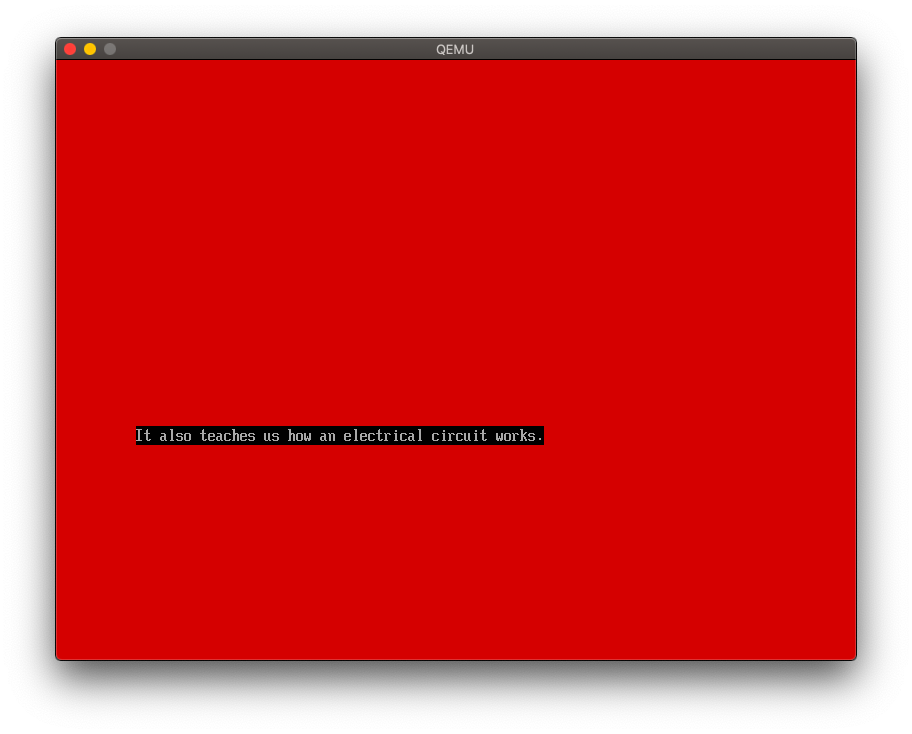
\includegraphics[scale=0.22]{pic/defaultfont.png}
            \caption{標準インターフェースでの文字の表示例}
            \label{fig:defaultfont}
        \end{minipage}
        \begin{minipage}{0.5\hsize}
            \centering
            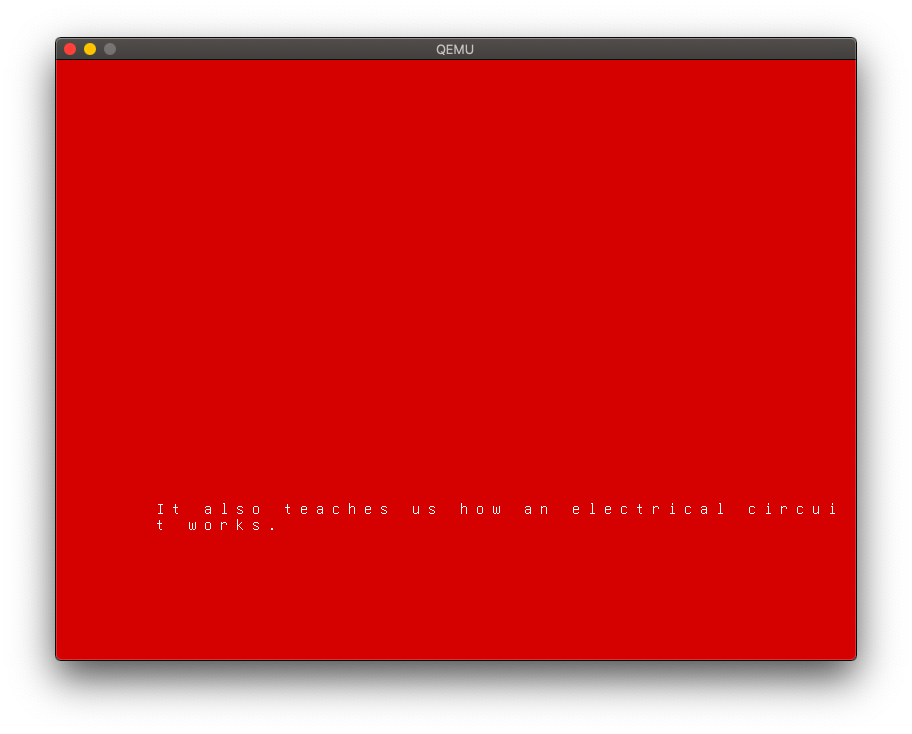
\includegraphics[scale=0.22]{pic/screenshot.png}
            \caption{透過処理を施したビットマップフォントでの文字の表示例}
            \label{fig:bitmapfont}
        \end{minipage}
    \end{tabular}  
\end{figure}
今回はGNU Unifontのビットマップ画像を用いたフォント表示を実装することにしました。
ビットマップフォントなので見た目はよろしくありませんが、背景色を透過できるためより自然な見た目になります。
\footnote{将来的にはTrueTypeフォントを扱えるようにすることでより綺麗にフォントが表示したいです。誰かが既にやってそうですが…}

UEFIでの文字はUnicode(UTF-16)で扱われるので、各文字に対して上位ビットと下位ビットを抜き出すことで対応する範囲のフォントを表示しています。
例えばUTF-16での「あ」は0x3042で表現でき、上位ビットは0x30、下位ビットは0x42と分解できます。
ここからビットマップ上の座標へと変換して表示しています。

また、長い文章などを表示する際はビデオディスプレイの幅からはみ出さないように適切な位置で折り返す必要があります。
これは次に入力される文字がディスプレイの幅からはみ出す場合に行を変えることで実装ができます(例えば以下のように)。
\begin{lstlisting}[style=customC,caption=Wrap around process,label=prog:wraparound]
for(UINT8 i = 0; i < length; i++, PrintPosX += FontDiv){
    CHAR16 tmp = string[i];
    UINT8 msb = (tmp & 0xFF00) >> 8, lsb = tmp & 0x00FF;
    if(PrintPosX + FontDiv > DispWidth){
        PrintPosY += FontDiv;
        PrintPosX = x;
    }
    WriteToBuffer(Go, Fonts, BltBuffer, Width, Height, Bpp, XOffset + FontDiv * lsb, YOffset + FontDiv * msb, FontDiv, FontDiv, PrintPosX, PrintPosY, MASK);
}
\end{lstlisting}
この例では文字を表示する際のX座標(PrintPosX)と文字幅(FontDiv)がディスプレイの幅(DispWidth)よりも大きい場合に改行するコードです。
GNU Unifontは縦横16 pixelの等幅フォントなので非常に簡素な実装で実現できます。
\footnote{プロポーショナルフォントでもそこまで難しくはならないとは思いますが}

\section{キー処理}
キー入力はReadKeyStroke関数を用いることで取得することが可能です。
ReadKeyStroke関数を実行すると\verb+EFI_INPUT_KEY+構造体に関数実行時点での入力キーが代入されます。
\verb+EFI_INPUT_KEY+構造体は以下のように定義されます。
\begin{lstlisting}[caption=EFI\_INPUT\_KEY,label=efi_input_key]
typedef struct {
    unsigned short ScanCode;
    unsigned short UnicodeChar;
} EFI_INPUT_KEY;
\end{lstlisting}
ScanCodeはUnicodeで表現できない文字が入力された場合に格納される変数です。
例えばEscキーが入力されるとScanCodeには0x17(23)が代入されます。
UTF-16で表現できる場合は0が代入されます。

UnicodeCharはScanCodeとは逆にUnicodeで表現できる文字が入力された場合に対応する文字を代入します。
Unicodeで表現できない文字の場合は0を代入します。

\chapter{あとがき}
始めに、ここまで読んでいただきありがとうございます。
そもそものきっかけが自分だけの本を何か出したいなあというのが動機だったので、内容が薄っぺらい感じの本になってしまった感あります。
ただ本を書くという経験自体は結構楽しくできたので(締切前はしんどかったですが…)個人的には良い経験が出来たと思っています。
続きの本を出すかは執筆段階では決めていませんが、他にも色々なジャンルで挑戦してみたいとは思っています
(そもそも碌にブログすら更新していないのでまずはそっちをやらねば…という気持ちです)。

UEFIを題材に選んだ理由は単純に低レイヤ(と言っていいのかは分かりませんが)に興味があったのと、UEFI-DOOM
\footnote{https://github.com/warfish/DOOM}
を見てDOOMが動かせるなら他のゲームとかも動かせるんじゃね?と思ったのが主な理由です。
実際には仕様書の長さに唖然としたり(2500ページ超)、コードのデバッグがうまくできずにしばらく放置していたり(これは自分の性格的な問題もありますが)とこの程度の内容を書くのにさえ色々難航した部分があったりとまだまだ完成には程遠い所にいるとは感じています
(BGM機能とか手を付けれてすらいないですし…)。
なのでこの本で終わりにするつもりは全く無く、今後も気長に進めていければと思います。
コンスタントに本出したりモノ作ってる人、やっぱり他の人とは違う何かがあるんだろうか…。

今後で一番やりたいのはBGM回りの実装とフォントレンダリングを真面目にやりたいと考えています。
(ぶっちゃけ今のフォントだと見栄えもあったもんじゃないので…)

というわけで、次また出す機会があればよろしくお願い致します。
\newpage

\thispagestyle{empty}
\printbibliography[title=参考文献]
\newpage

% 奥付
\thispagestyle{empty}
\vspace*{\stretch{1}}
\begin{flushright}
    \begin{minipage}{0.8\hsize}
        \begin{description}
            \item{タイトル: } hogehogehoge
            \item{著者: }こめわっぽ
            \item{発行: }2019年8月12日
            \item{連絡先: }komekome09.online@gmail.com
            \item{Twitter: }@komekome09
            \item{印刷: }株式会社 栄光 様
        \end{description}
    \end{minipage}
\end{flushright}
\newpage

% 裏表紙裏
\thispagestyle{empty}
\mbox{}
\newpage

\end{document}

